\chapter{Architecture}
 
\begin{figure}[!h]
\begin{center}
  \fbox{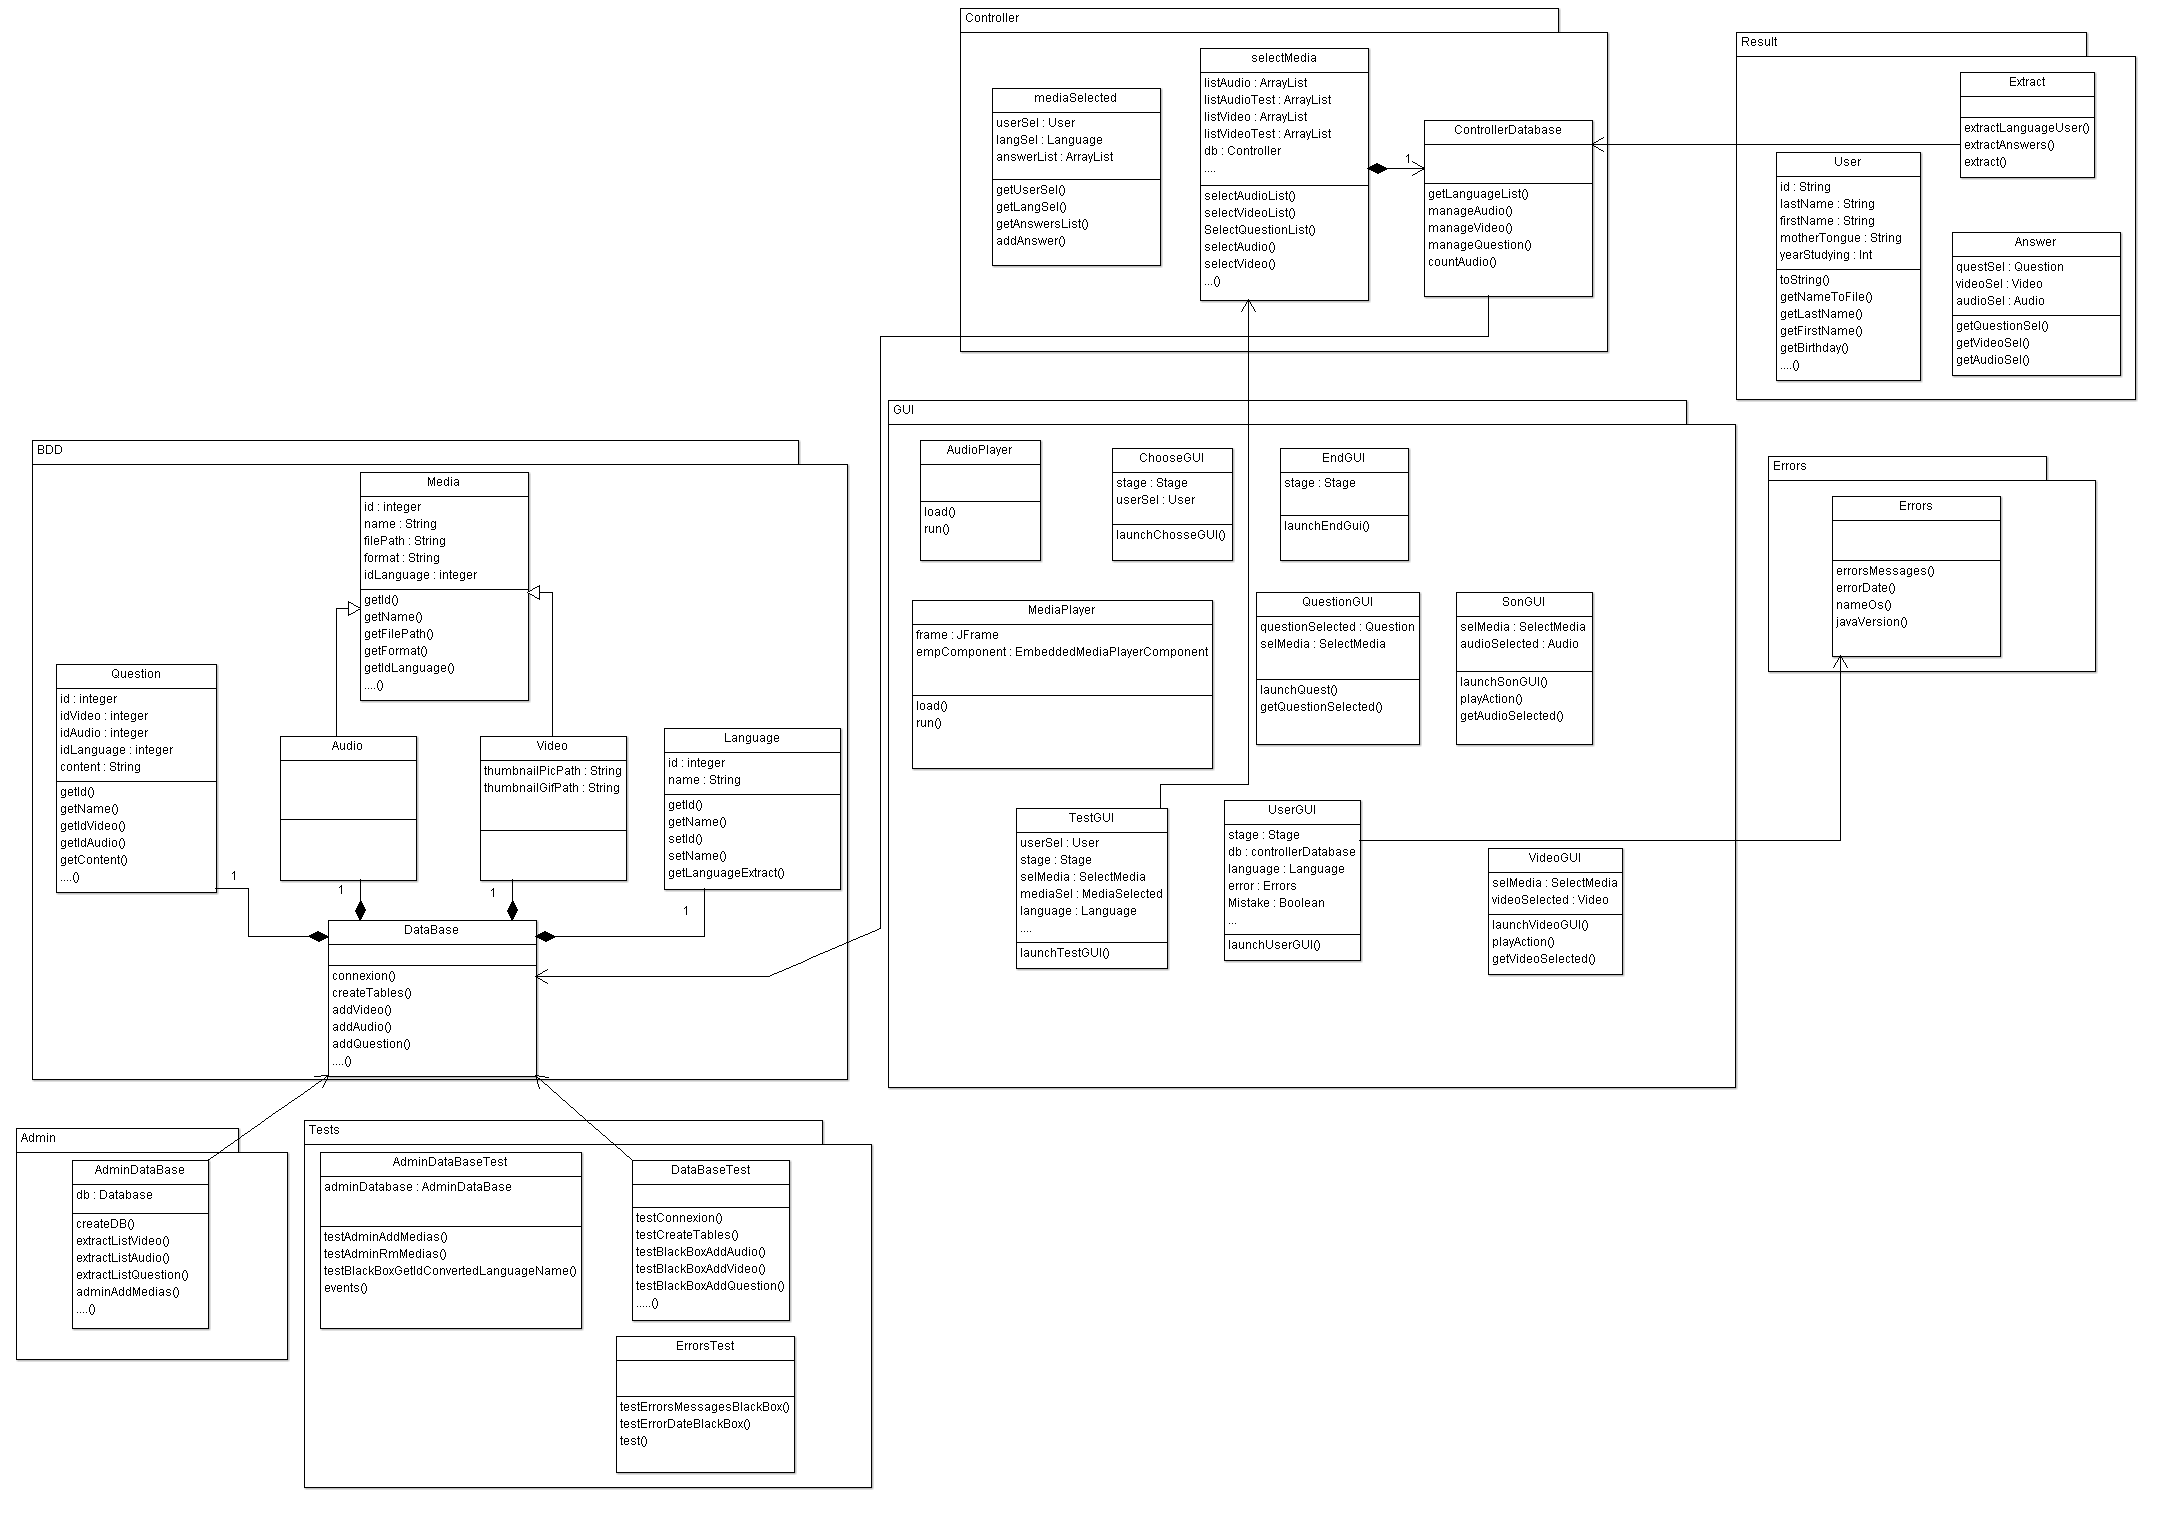
\includegraphics[width=18cm,angle=90]{./architecture/architecture.png}}
  \caption{UML - Architecture}
  \label{diaglog} 
\end{center}
\end{figure}

Notre architecture est de type MVC. Le pattern MVC nous a permis de bien organiser notre code source. Il nous a aidé à connaitre quels fichiers créés et à bien définir leur fonction. Grâce à ce \textit{design pattern}, on a pu répartir les rôles de chacun afin de produire un travail soigné.

\section{Explication détaillée des packages}

Notre architecture est structuré en plusieurs packages. Ils ont été créés avec comme but de séparer notre architecture en fonction des besoins renseignés précédemment. Chaque package regroupe un certain nombre de classe possédant chacune une fonction bien précise. Dans cette section, nous allons décrire le besoin que nous avons voulu satisfaire avec le package et le rôle de chaque classe contenue dans le package.

\subsection{BDD}

On a créer ce package afin de regrouper les classes qui nous permette de gérer les données que va utiliser l'application. Ces données sont en lien avec la base de données que nous avons créé. Elle est consituée plusieurs entités comme les vidéos, les audios, les questions et enfin les langues. Cette organisation des données a été choisie pour satisfaire et optimiser l'ajout de médias. De plus, si dans un futur proche, notre client souhaite intégrer une nouvelle langue pour ces tests, cet ajout sera simple et rapide.\\
Dans notre architecture, ce package correspond à la partie \textit{modèle}.

\subsubsection{Classe DataBase}

Cette classe est très importante dans notre application. En effet, c'est le lien entre l'application et la base de données. La procédure "connexion" sert à la création, si celle-ci n'existe pas, et à la connexion avec la base de données. La procédure "createTable" crée les tables nécessaires au fonctionnement de notre application si celles-ci ne le sont déjà pas. Nous avons mis en place diverses autres fonctions qui nous permettent d'ajouter, de gérer et de supprimer videos, audios, questions et langues de notre base de données. De plus, diverses autres méthodes ont été implémentées pour nous faciliter les implémentations de notre application, comme par exemple les fonctions qui nous retourne une liste d'objet correspondant aux médias de la base de données selon la langue.

\subsubsection{Classes Media, Audio et Video}

Ces trois classes sont unis. Effectivement, les classes \textit{Audio} et \textit{Video} héritent de la classe abstraite \textit{Media}. Cette dernière regroupe les méthodes communes aux classes héritées. Celles-ci sont importantes dans notre application puisqu'elles créent les objets en fonction du contenu de la base de données. Ils serviront pour la lecture des médias dans notre application grâce aux "path" renseignés dans la base données.

\subsubsection{Classe Question, Language}

Ces classes créent des objets correspondant à une question, à une langue ; chacune provenant de la base de données. Les langues nous permettrons de sélectionner les questions, audios et vidéos qui seront proposés à l'utilisateur de l'application. 

\subsection{Result}

Ce package a pour fonction de regrouper les classes qui seront utiles pour l'étude de notre client. Il est constitué d'une classe qui rassemble les informations nécessaires de l'utilisateur, d'une autre qui liste les réponses de celui-ci effectuées lors du test et enfin d'une classe qui extrait toutes ces données dans un fichier.

\subsubsection{Classe User}

Cette classe se compose de différents attributs qui permettent de différencier chaque sujet. Tous ces renseignements nous ont été demandées par notre client afin qu'il puisse statistiquer les résultats.

\subsubsection{Classe Answer}

Cette classe regoupe un trio d'objets composé de \textit{Question}, \textit{Audio} et \textit{Video} qui correspondent à la réponse audio et vidéo pour la question posée à l'utilisateur.

\subsubsection{Classe Extract}

Cette classe sert à extraire, dans un fichier, la langue du test, les données de l'utilisateur ainsi que les réponses de celui-ci. Elle n'est composée que de méthodes statiques. En effet, on a trouvé inutile de créer un objet pour cela vu que la méthode principale n'est appelée qu'une unique fois dans l'application. Chaque extraction est effectuée lorsque l'utilisateur valide sa dernière réponse.

\subsection{GUI}

Ce package regroupe toutes les configuration et les fonctionnalités de l'interface graphique. C'est le plus imposant de nos packages vu que notre application possède plusieurs interfaces différentes.\\
Dans notre architecture, ce package correspond à la partie \textit{vue}.

\subsubsection{Classe Start}

Cette classe est importante puisque c'est à partir de là que l'application se lance. Dans la fonction "Launch()", nous avons défini la taille de notre fenêtre (appelé Stage dans un environnement JavaFX) ainsi que son titre. Puis, nous avons configuré la feuille de style de la scène (qui correspond au container du stage). C'est le point de départ de notre interface. A partir de maintenant, il suffisait juste de "remplir" la scene avec les différents éléments.

\subsubsection{Classe UserGUI}

Cette classe correspond à l'interface graphique où l'utilisateur renseigne ces informations à l'aide des champs créer pour et sélectionne la langue du test. Les langues sont extraites de la base de données. Une fois tous renseignés, un objet de type \textit{User} est créé une fois le bouton "next" cliqué.

\subsubsection{Classe ChooseGUI}

Cette classe est simple étant donnée qu'il ne s'agit que de deux boutons qui permettent de choisir entre la session d'entrainement et la session test.

\subsubsection{Classe TestGUI}

Cette classe est assez spécial vu que plusieurs objets graphique gravite autour d'elle. En effet, on peut dire que l'interface qui en résulte est composé de quatre composants : l'audio, la vidéo, les question et les différents boutons pour le mix et la validation. La classe place tous ces objets dans le panel de la scene. 


\subsection{Processes}

Nous avons réuni ici, tout ce qui correspond au \textit{contrôleur} de l'application.

La classe \textbf{GUI\_select} est la sélection de l'ensemble des médias présentées lors d'une question.
\textbf{GUI\_Answer} correspond à la vidéo et à l'audio sélectionnés par l'utilisateur liés à une question.

\textbf{Cmd} est l'utilisation de l'application par l'administrateur lorsqu'il voudra ajouter ou retirer des médias et questions de la base de données.

\subsection{Tests}

Ce package regroupe l'ensemble des tests qui seront necessaires pour minimiser les erreurs au niveau de la base de données (par exemple lors d'un upload de médias, on vérifie que le format soit adapté).